\documentclass[journal,12pt,twocolumn]{IEEEtran}
%
\usepackage{setspace}
\usepackage{gensymb}
\singlespacing
\usepackage[cmex10]{amsmath}
\usepackage{siunitx}
\usepackage{amsthm}

\usepackage{mathrsfs}

\usepackage{txfonts}
\usepackage{stfloats}

\usepackage{steinmetz}
\usepackage{cite}
\usepackage{cases}
\usepackage{subfig}
\usepackage{longtable}
\usepackage{multirow}
\usepackage{enumitem}
\usepackage{mathtools}
\usepackage{tikz}
\usepackage{circuitikz}
\usepackage{verbatim}
\usepackage{tfrupee}
\usepackage[breaklinks=true]{hyperref}
\usepackage{tkz-euclide} % loads  TikZ and tkz-base
\usetikzlibrary{calc,math}
\usetikzlibrary{fadings}
\usepackage{listings}
    \usepackage{color}                                            %%
    \usepackage{array}                                            %%
    \usepackage{longtable}                                        %%
    \usepackage{calc}                                             %%
    \usepackage{multirow}                                         %%
    \usepackage{hhline}                                           %%
    \usepackage{ifthen}                                           %%
  %optionally (for landscape tables embedded in another document): %%
    \usepackage{lscape}     
\usepackage{multicol}
\usepackage{chngcntr}
\DeclareMathOperator*{\Res}{Res}

\renewcommand\thesection{\arabic{section}}
\renewcommand\thesubsection{\thesection.\arabic{subsection}}
\renewcommand\thesubsubsection{\thesubsection.\arabic{subsubsection}}

\renewcommand\thesectiondis{\arabic{section}}
\renewcommand\thesubsectiondis{\thesectiondis.\arabic{subsection}}
\renewcommand\thesubsubsectiondis{\thesubsectiondis.\arabic{subsubsection}}

\hyphenation{op-tical net-works semi-conduc-tor}
\def\inputGnumericTable{}                                 %%

\lstset{
%language=C,
frame=single, 
breaklines=true,
columns=fullflexible
}
\begin{document}
%


\newtheorem{theorem}{Theorem}[section]
\newtheorem{problem}{Problem}
\newtheorem{proposition}{Proposition}[section]
\newtheorem{lemma}{Lemma}[section]
\newtheorem{corollary}[theorem]{Corollary}
\newtheorem{example}{Example}[section]
\newtheorem{definition}[problem]{Definition}
\newcommand{\BEQA}{\begin{eqnarray}}
\newcommand{\EEQA}{\end{eqnarray}}
\newcommand{\define}{\stackrel{\triangle}{=}}
\bibliographystyle{IEEEtran}
\providecommand{\mbf}{\mathbf}
\providecommand{\pr}[1]{\ensuremath{\Pr\left(#1\right)}}
\providecommand{\qfunc}[1]{\ensuremath{Q\left(#1\right)}}
\providecommand{\sbrak}[1]{\ensuremath{{}\left[#1\right]}}
\providecommand{\lsbrak}[1]{\ensuremath{{}\left[#1\right.}}
\providecommand{\rsbrak}[1]{\ensuremath{{}\left.#1\right]}}
\providecommand{\brak}[1]{\ensuremath{\left(#1\right)}}
\providecommand{\lbrak}[1]{\ensuremath{\left(#1\right.}}
\providecommand{\rbrak}[1]{\ensuremath{\left.#1\right)}}
\providecommand{\cbrak}[1]{\ensuremath{\left\{#1\right\}}}
\providecommand{\lcbrak}[1]{\ensuremath{\left\{#1\right.}}
\providecommand{\rcbrak}[1]{\ensuremath{\left.#1\right\}}}
\theoremstyle{remark}
\newtheorem{rem}{Remark}
\newcommand{\sgn}{\mathop{\mathrm{sgn}}}
\providecommand{\abs}[1]{\left\vert#1\right\vert}
\providecommand{\abs}[1]{\lvert#1\rvert} 
\providecommand{\res}[1]{\Res\displaylimits_{#1}} 
\providecommand{\norm}[1]{\left\lVert#1\right\rVert}
%\providecommand{\norm}[1]{\lVert#1\rVert}
\providecommand{\mtx}[1]{\mathbf{#1}}
\providecommand{\mean}[1]{E\left[ #1 \right]}
\providecommand{\fourier}{\overset{\mathcal{F}}{ \rightleftharpoons}}
%\providecommand{\hilbert}{\overset{\mathcal{H}}{ \rightleftharpoons}}
\providecommand{\system}{\overset{\mathcal{H}}{ \longleftrightarrow}}
	%\newcommand{\solution}[2]{\textbf{Solution:}{#1}}
\newcommand{\solution}{\noindent \textbf{Solution: }}
\newcommand{\cosec}{\,\text{cosec}\,}
\providecommand{\dec}[2]{\ensuremath{\overset{#1}{\underset{#2}{\gtrless}}}}
\newcommand{\myvec}[1]{\ensuremath{\begin{pmatrix}#1\end{pmatrix}}}
\newcommand{\mydet}[1]{\ensuremath{\begin{vmatrix}#1\end{vmatrix}}}
\numberwithin{equation}{subsection}
\makeatletter
\@addtoreset{figure}{problem}
\makeatother
\let\StandardTheFigure\thefigure
\let\vec\mathbf
\renewcommand{\thefigure}{\theproblem}
\def\putbox#1#2#3{\makebox[0in][l]{\makebox[#1][l]{}\raisebox{\baselineskip}[0in][0in]{\raisebox{#2}[0in][0in]{#3}}}}
     \def\rightbox#1{\makebox[0in][r]{#1}}
     \def\centbox#1{\makebox[0in]{#1}}
     \def\topbox#1{\raisebox{-\baselineskip}[0in][0in]{#1}}
     \def\midbox#1{\raisebox{-0.5\baselineskip}[0in][0in]{#1}}
\vspace{3cm}
\title{ASSIGNMENT-15}
\author{R.YAMINI}
\maketitle
\newpage
\bigskip
\renewcommand{\thefigure}{\theenumi}
\renewcommand{\thetable}{\theenumi}


%
\section{QUESTION No-2.9(Optimization)}
Find the maximum area of an isosceles triangle inscribed in the ellipse $\vec{x}^{\top}\myvec{a^2 & 0 \\ 0 & b^2}\vec{x} = a^2b^2$
with its vertex at one end of the major axis.
\section{Solution}
Let $OD=y$ and $BD=x$. From the below figure we obtain the
\numberwithin{figure}{section}
\begin{figure}[!ht]
\centering
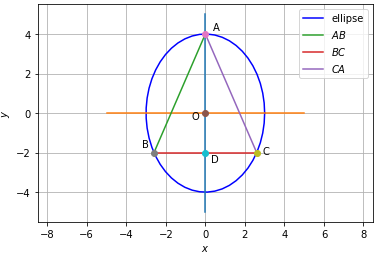
\includegraphics[width=\columnwidth]{isosceles.PNG}
\caption{isosceles triangle inscribed in the ellipse}
\label{fig:Graph}	
\end{figure}
area of the $\triangle ABC$ as, 
\begin{align}
    \frac{1}{2}\mydet{\vec{B}-\vec{C}}\mydet{\vec{A}-\vec{D}} &=x(a+y)
\end{align}
Now the objective function is given as
\begin{align}
    \max Z = ax+xy
\end{align}
subject to constraint
\begin{align}
    \vec{x}^{\top}\myvec{a^2 & 0 \\ 0 & b^2}\vec{x}-a^2b^2=0.\label{eq6}
\end{align}
Let
\begin{align}
    f(x,y)=ax+xy \\
    g(x,y)=\vec{x}^{\top}\myvec{a^2 & 0 \\ 0 & b^2}\vec{x}-a^2b^2
\end{align}
and we solve this using Lagrange multipliers,
\begin{align}
    \nabla \vec{f} = \lambda\brak{\nabla \vec{g}} \\ 
    \myvec{a+y \\ x} = \lambda \myvec{2a^2x \\ 2b^2y} \label{eq1}
\end{align}
we obtain the following from \eqref{eq1}
\begin{align}
    a+y=2\lambda a^2x \label{eq2} \\ 
    x= 2\lambda b^2y \label{eq3} \\
    \implies \lambda = \frac{x}{2b^2y} \label{eq4}
\end{align}
substitute \eqref{eq3} in \eqref{eq2}
\begin{align}
    a+y = 2\lambda a^2\brak{2\lambda b^2y} \label{eq5}
\end{align}    
now substitute \eqref{eq4} in \eqref{eq5}
\begin{align}
    a+y = \frac{x^2a^2}{b^2y} \label{eq7}
\end{align}
using \eqref{eq6} in \eqref{eq7} we have,
\begin{align}
  ab^2y+2b^2y^2=a^2b^2 \\
  \implies 2y^2+ay-a^2=0 \\
  \implies y = -a ,\frac{1}{2}a.
\end{align}
We see that $y=-a$ doesn't give any value for $x$ so substitute $y=\frac{1}{2}a$ in \eqref{eq7},
\begin{align}
    a+\brak{\frac{1}{2}a} = \frac{x^2a^2}{b^2\brak{\frac{1}{2}a}}
    \\ \implies x^2 = \frac{3ab^2}{4} \\
    \implies x= \frac{(\sqrt{3a})b}{2}.
\end{align}
Thus we obtain $\vec{x} = \myvec{\frac{(\sqrt{3a})b}{2} \\ \frac{1}{2}a}$. Hence we obtain
\begin{equation}
\begin{aligned}
    Z &= a\brak{\frac{(\sqrt{3a})b}{2}} + \frac{(\sqrt{3a})b}{2} \brak{\frac{1}{2}a} \\
    &= \frac{3\sqrt{3}ab}{4}.
\end{aligned}
\end{equation}
Thus the maximum area of the isosceles triangle inscribed in ellipse is $\frac{3\sqrt{3}ab}{4}.$


\end{document}
